% questions.tex —— 2013 年·重庆卷·理科 · 题目内容片段（无答案）
% 由 tools/generate_projects.py 依来源总账自 2013/2013_数学真题_重庆理_试题.md 生成，勿手改（改源 MD 后重跑）


\begin{gknotice}
\textbf{来源说明}：本题面依据固定源 PDF 的两页 A3 题面逐题转录，原卷印刷页码为 791–792。第 791 面为选择题 1—10、填空题 11—16、解答题 17—18，第 792 面为解答题 19—22；原卷第 15、16 题为极坐标与不等式题，与其余填空题连续编号，无选做标记。

\textbf{解析归属}：固定源不附答案或解析；配套答案与解析均由本库按本题面独立复算。

\textbf{图形说明}：第 4 题茎叶图、第 5 题三视图、第 8 题程序框图、第 14 题圆与切线、第 19 题四棱锥、第 21 题椭圆与圆 Q 均由项目内 TikZ 矢量源重绘。
\end{gknotice}

\gkpart{一、选择题}

\begin{question}
\gkti{1}已知全集 $U=\{1,2,3,4\}$，集合 $A=\{1,2\}$，$B=\{2,3\}$，则 $\complement_U(A\cup B)=$\mbox{（　　）}

（A）$\{1,3,4\}$；（B）$\{3,4\}$；（C）$\{3\}$；（D）$\{4\}$。

\end{question}
\begin{question}
\gkti{2}命题“对任意 $x\in\mathbf R$，都有 $x^2\geqslant0$”的否定为\mbox{（　　）}

（A）对任意 $x\in\mathbf R$，都有 $x^2<0$；（B）不存在 $x\in\mathbf R$，使得 $x^2<0$；（C）存在 $x_0\in\mathbf R$，使得 $x_0^2\geqslant0$；（D）存在 $x_0\in\mathbf R$，使得 $x_0^2<0$。

\end{question}
\begin{question}
\gkti{3}$\sqrt{(3-a)(a+6)}$（$-6\leqslant a\leqslant3$）的最大值为\mbox{（　　）}

（A）$9$；（B）$\dfrac92$；（C）$3$；（D）$\dfrac{3\sqrt2}2$。

\Needspace{0.4\textheight}
\end{question}
\begin{question}
\gkti{4}以下茎叶图记录了甲、乙两组各 $5$ 名学生在一次英语听力测试中的成绩（单位：分）。
\nopagebreak[4]
\begin{center}% 2013 重庆卷理科第 4 题：甲、乙两组各 5 名学生听力成绩的茎叶图。
% 茎（十位）为中间的 0、1、2；甲组叶在左、乙组叶在右。
% 甲组数据 9，1x，12，27，24；乙组数据 9，15，1y，18，24。
\begin{tikzpicture}[font=\small, line width=0.45pt, x=0.62cm, y=0.72cm]
  % 表头
  \node[anchor=east] at (-0.85,3.95) {甲组};
  \node[anchor=west] at (0.85,3.95) {乙组};
  \draw (-2.35,3.55) -- (3.45,3.55);
  % 茎列的两条竖线
  \draw (-0.55,3.55) -- (-0.55,0.55);
  \draw (0.55,3.55) -- (0.55,0.55);
  % 三行：茎 0、1、2
  \node at (0,3.0) {0};
  \node at (0,2.15) {1};
  \node at (0,1.3) {2};
  % 甲组叶
  \node[anchor=east] at (-0.85,3.0) {9};
  \node[anchor=east] at (-0.85,2.15) {$x$\ \ 2};
  \node[anchor=east] at (-0.85,1.3) {7\ \ 4};
  % 乙组叶
  \node[anchor=west] at (0.85,3.0) {9};
  \node[anchor=west] at (0.85,2.15) {5\ \ $y$\ \ 8};
  \node[anchor=west] at (0.85,1.3) {4};
\end{tikzpicture}
\end{center}
\nopagebreak[4]
已知甲组数据的中位数为 $15$，乙组数据的平均数为 $16.8$，则 $x$，$y$ 的值分别为\mbox{（　　）}

（A）$2$，$5$；（B）$5$，$5$；（C）$5$，$8$；（D）$8$，$8$。

\Needspace{0.4\textheight}
\end{question}
\begin{question}
\gkti{5}某几何体的三视图如图所示，则该几何体的体积为\mbox{（　　）}
\nopagebreak[4]
\begin{center}% 2013 重庆卷理科第 5 题：几何体的三视图。
% 正（主）视图为 10×4 的矩形；侧（左）视图为下底 8、上底 2、高 4 的等腰梯形；
% 俯视图为 10×8 的矩形，被两条与长边平行的线分成 3、2、3 三部分。
\begin{tikzpicture}[font=\small, >=Stealth, line width=0.45pt, x=0.26cm, y=0.26cm]
  % ---- 正（主）视图：10 宽、4 高 ----
  \draw (0,0) rectangle (10,4);
  \draw[<->] (-2,0) -- (-2,4);
  \draw (-2.8,0) -- (-1.2,0);
  \draw (-2.8,4) -- (-1.2,4);
  \node[left] at (-2.8,2) {4};
  \draw[<->] (0,-2) -- (10,-2);
  \draw (0,-2.8) -- (0,-1.2);
  \draw (10,-2.8) -- (10,-1.2);
  \node[below] at (5,-2.2) {10};
  \node[below] at (5,-3.8) {正（主）视图};

  % ---- 侧（左）视图：下底 8、上底 2、高 4 的等腰梯形 ----
  \begin{scope}[shift={(13.6,0)}]
    \draw (0,0) -- (8,0) -- (5,4) -- (3,4) -- cycle;
    \draw[<->] (0,-2) -- (8,-2);
    \draw (0,-2.8) -- (0,-1.2);
    \draw (8,-2.8) -- (8,-1.2);
    \node[below] at (4,-2.2) {8};
    \node[below] at (4,-3.8) {侧（左）视图};
  \end{scope}

  % ---- 俯视图：10×8 的矩形，分成 3、2、3 ----
  \begin{scope}[shift={(0,-15.4)}]
    \draw (0,0) rectangle (10,8);
    \draw (0,5) -- (10,5);
    \draw (0,3) -- (10,3);
    \draw[<->] (-2,0) -- (-2,3);
    \draw[<->] (-2,3) -- (-2,5);
    \draw[<->] (-2,5) -- (-2,8);
    \draw (-2.8,0) -- (-1.2,0);
    \draw (-2.8,3) -- (-1.2,3);
    \draw (-2.8,5) -- (-1.2,5);
    \draw (-2.8,8) -- (-1.2,8);
    \node[left] at (-2.8,1.5) {3};
    \node[left] at (-2.8,4) {2};
    \node[left] at (-2.8,6.5) {3};
    \node[below] at (5,-1.4) {俯视图};
  \end{scope}
\end{tikzpicture}
\end{center}
\nopagebreak[4]
（A）$\dfrac{560}3$；（B）$\dfrac{580}3$；（C）$200$；（D）$240$。

\end{question}
\begin{question}
\gkti{6}若 $a<b<c$，则函数 $f(x)=(x-a)(x-b)+(x-b)(x-c)+(x-c)(x-a)$ 的两个零点分别位于区间\mbox{（　　）}

（A）$(a,b)$ 和 $(b,c)$ 内；（B）$(-\infty,a)$ 和 $(a,b)$ 内；（C）$(b,c)$ 和 $(c,+\infty)$ 内；（D）$(-\infty,a)$ 和 $(c,+\infty)$ 内。

\end{question}
\begin{question}
\gkti{7}已知圆 $C_1:(x-2)^2+(y-3)^2=1$，圆 $C_2:(x-3)^2+(y-4)^2=9$，$M$，$N$ 分别是圆 $C_1$，$C_2$ 上的动点，$P$ 为 $x$ 轴上的动点，则 $|PM|+|PN|$ 的最小值为\mbox{（　　）}

（A）$5\sqrt2-4$；（B）$\sqrt{17}-1$；（C）$6-2\sqrt2$；（D）$\sqrt{17}$。

\Needspace{0.4\textheight}
\end{question}
\begin{question}
\gkti{8}执行如图所示的程序框图，如果输出 $s=3$，那么判断框内应填入的条件是\mbox{（　　）}
\nopagebreak[4]
\begin{center}% 2013 重庆卷理科第 8 题：程序框图。
% k=2，s=1；循环体 s=s·log_k(k+1)，k=k+1；判断框为“是”时返回循环，为“否”时输出 s。
\begin{tikzpicture}[font=\small, >=Stealth, line width=0.5pt,
    block/.style={draw, rectangle, minimum width=2.8cm, minimum height=0.8cm, inner sep=3pt},
    wide/.style={draw, rectangle, minimum width=5.7cm, minimum height=0.95cm, inner sep=3pt},
    term/.style={draw, rectangle, rounded corners=4pt, minimum width=1.7cm, minimum height=0.75cm, inner sep=3pt},
    io/.style={draw, trapezium, trapezium left angle=72, trapezium right angle=108,
      minimum width=2.6cm, minimum height=0.85cm, inner sep=3pt},
    dec/.style={draw, diamond, aspect=2.6, minimum width=4.6cm, minimum height=1.9cm, inner sep=1pt}]
  \node[term] (start) at (0,9.3) {开始};
  \node[wide] (init) at (0,7.8) {$k=2$,\ $s=1$};
  \node[wide] (loop) at (0,6.1) {$s=s\cdot\log_k(k+1)$};
  \node[block] (inc) at (0,4.35) {$k=k+1$};
  \node[dec] (test) at (0,2.5) {};
  \node[io] (out) at (0,0.75) {输出 $s$};
  \node[term] (stop) at (0,-0.6) {结束};

  \draw[->] (start) -- (init);
  \draw[->] (init) -- (loop);
  \draw[->] (loop) -- (inc);
  \draw[->] (inc) -- (test);
  \draw[->] (test) -- node[left, pos=0.45] {否} (out);
  \draw[->] (out) -- (stop);
  % 是：回到循环体上方
  \draw[->] (test.east) -- (4.3,2.5) -- (4.3,6.95) -- node[above, pos=0.75] {是} (0,6.95);
\end{tikzpicture}
\end{center}
\nopagebreak[4]
（A）$k\leqslant6$；（B）$k\leqslant7$；（C）$k\leqslant8$；（D）$k\leqslant9$。

\end{question}
\begin{question}
\gkti{9}$4\cos50^\circ-\tan40^\circ=$\mbox{（　　）}

（A）$\sqrt2$；（B）$\dfrac{\sqrt2+\sqrt3}2$；（C）$\sqrt3$；（D）$2\sqrt2-1$。

\end{question}
\begin{question}
\gkti{10}在平面上，$\overrightarrow{AB_1}\perp\overrightarrow{AB_2}$，$|\overrightarrow{OB_1}|=|\overrightarrow{OB_2}|=1$，$\overrightarrow{AP}=\overrightarrow{AB_1}+\overrightarrow{AB_2}$。若 $|\overrightarrow{OP}|<\dfrac12$，则 $|\overrightarrow{OA}|$ 的取值范围是\mbox{（　　）}

（A）$\left(0,\dfrac{\sqrt5}2\right]$；（B）$\left(\dfrac{\sqrt5}2,\dfrac{\sqrt7}2\right]$；（C）$\left(\dfrac{\sqrt5}2,\sqrt2\right]$；（D）$\left(\dfrac{\sqrt7}2,\sqrt2\right]$。

\end{question}
\begingroup
\renewcommand{\gkpart}[1]{\Needspace{0.2\textheight}\subsection*{#1}\nopagebreak}
\gkpart{二、填空题}
\endgroup

\begin{question}
\gkti{11}已知复数 $z=\dfrac{5\mathrm i}{1+2\mathrm i}$（$\mathrm i$ 是虚数单位），则 $|z|=$\gkblank{}。

\end{question}
\begin{question}
\gkti{12}已知 $\{a_n\}$ 是等差数列，$a_1=1$，公差 $d\neq0$，$S_n$ 为其前 $n$ 项和，若 $a_1$，$a_2$，$a_5$ 成等比数列，则 $S_8=$\gkblank{}。

\end{question}
\begin{question}
\gkti{13}从 $3$ 名骨科、$4$ 名脑外科和 $5$ 名内科医生中选派 $5$ 人组成一个抗震救灾医疗小组，则骨科、脑外科和内科医生都至少有 $1$ 人的选派方法种数是\gkblank{}（用数字作答）。

\Needspace{0.4\textheight}
\end{question}
\begin{question}
\gkti{14}如图，在 $\triangle ABC$ 中，$\angle C=90^\circ$，$\angle A=60^\circ$，$AB=20$，过 $C$ 作 $\triangle ABC$ 的外接圆的切线 $CD$，$BD\perp CD$，$BD$ 与外接圆交于点 $E$，则 $DE$ 的长为\gkblank{}。
\nopagebreak[4]
\begin{center}% 2013 重庆卷理科第 14 题：直角三角形外接圆与切线。
% ∠C=90°，∠A=60°，AB=20 为外接圆直径；CD 切圆于 C，BD⊥CD 于 D，BD 与圆交于 E。
% 图中取圆半径 3（即 10 按 0.3 缩放），C 在最下方，A 在左下，B 在右上，E 在 B、D 之间。
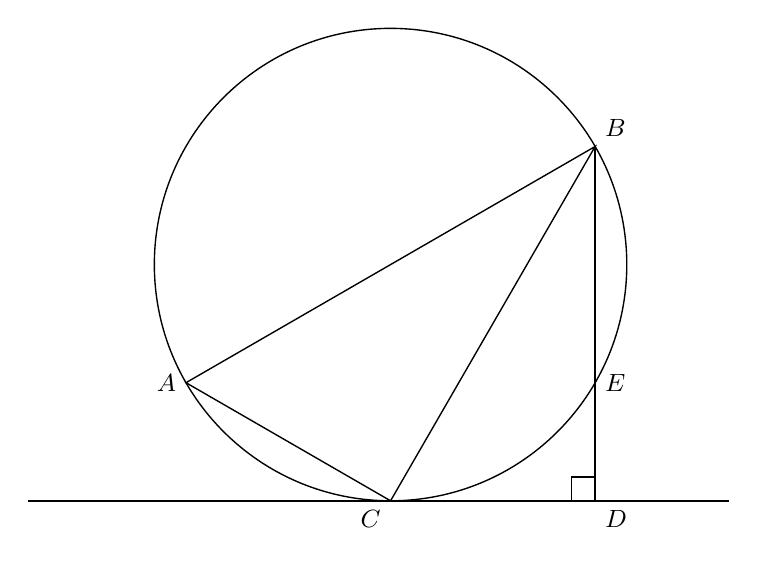
\begin{tikzpicture}[font=\small, line width=0.5pt, scale=1]
  \coordinate (O) at (0,0);
  \coordinate (C) at (0,-3);
  \coordinate (A) at (-2.5981,-1.5);
  \coordinate (B) at (2.5981,1.5);
  \coordinate (D) at (2.5981,-3);
  \coordinate (E) at (2.5981,-1.5);
  \draw (O) circle (3);
  % 切线 CD
  \draw (-4.6,-3) -- (4.3,-3);
  % 三角形与垂线
  \draw (A) -- (B) -- (C) -- cycle;
  \draw (B) -- (D);
  \draw (C) -- (D);
  % 直角标记（∠BCD 处，BC 与 CD 之间）
  \draw (2.5981,-2.7) -- (2.2981,-2.7) -- (2.2981,-3);
  \node[below left] at (C) {$C$};
  \node[left] at (A) {$A$};
  \node[above right] at (B) {$B$};
  \node[below right] at (D) {$D$};
  \node[right] at (E) {$E$};
\end{tikzpicture}
\end{center}
\nopagebreak[4]
\end{question}
\begin{question}
\gkti{15}在直角坐标系 $xOy$ 中，以原点 $O$ 为极点，$x$ 轴的正半轴为极轴建立极坐标系。若极坐标方程为 $\rho\cos\theta=4$ 的直线与曲线 $\begin{cases}x=t^2,\\y=t^3\end{cases}$（$t$ 为参数）相交于 $A$，$B$ 两点，则 $|AB|=$\gkblank{}。

\end{question}
\begin{question}
\gkti{16}若关于实数 $x$ 的不等式 $|x-5|+|x+3|<a$ 无解，则实数 $a$ 的取值范围是\gkblank{}。

\end{question}
\begingroup
\renewcommand{\gkpart}[1]{\Needspace{0.2\textheight}\subsection*{#1}\nopagebreak}
\gkpart{三、解答题}
\endgroup

\begin{question}
\gkti{17}设 $f(x)=a(x-5)^2+6\ln x$，其中 $a\in\mathbf R$，曲线 $y=f(x)$ 在点 $(1,f(1))$ 处的切线与 $y$ 轴相交于点 $(0,6)$。

（1） 确定 $a$ 的值；

（2） 求函数 $f(x)$ 的单调区间与极值。

\end{question}
\begin{question}
\gkti{18}某商场举行的“三色球”购物摸奖活动规定：在一次摸奖中，摸奖者先从装有 $3$ 个红球与 $4$ 个白球的袋中任意摸出 $3$ 个球，再从装有 $1$ 个蓝球与 $2$ 个白球的袋中任意摸出 $1$ 个球，根据摸出 $4$ 个球中红球与蓝球的个数，设一、二、三等奖如下：

\begin{center}
\begin{tabular}{lll}
\toprule
奖级 & 摸出红、蓝球个数 & 获奖金额 \\
\midrule
一等奖 & $3$ 红 $1$ 蓝 & $200$ 元 \\
二等奖 & $3$ 红 $0$ 蓝 & $50$ 元 \\
三等奖 & $2$ 红 $1$ 蓝 & $10$ 元 \\
\bottomrule
\end{tabular}
\end{center}

其余情况无奖且每次摸奖最多只能获得一个奖级。

（1） 求一次摸球恰好摸到 $1$ 个红球的概率；

（2） 求摸奖者在一次摸奖中获奖金额 $X$ 的分布列与期望 $E(X)$。

\Needspace{0.4\textheight}
\end{question}
\begin{question}
\gkti{19}如图，四棱锥 $P-ABCD$ 中，$PA\perp$ 底面 $ABCD$，$BC=CD=2$，$AC=4$，$\angle ACB=\angle ACD=\dfrac\pi3$，$F$ 为 $PC$ 的中点，$AF\perp PB$。

（1） 求 $PA$ 的长；

（2） 求二面角 $B-AF-D$ 的正弦值。
\nopagebreak[4]
\begin{center}% 2013 重庆卷理科第 19 题：四棱锥 P-ABCD。
% PA⊥底面 ABCD；BC=CD=2，AC=4，∠ACB=∠ACD=60°，F 为 PC 中点。
% 底面按斜二测示意绘制：A 在左，B 在下，C 在右，D 在右上；AD、AC、BD 为不可见棱。
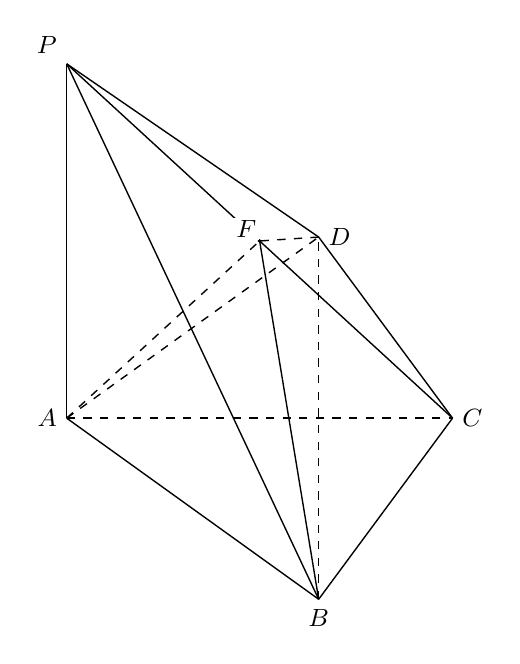
\begin{tikzpicture}[font=\small, line width=0.5pt, scale=1]
  \coordinate (A) at (0,0);
  \coordinate (P) at (0,4.5);
  \coordinate (B) at (3.2,-2.3);
  \coordinate (C) at (4.9,0);
  \coordinate (D) at (3.2,2.3);
  \coordinate (F) at (2.45,2.25);

  % 不可见棱
  \draw[dashed] (A) -- (D);
  \draw[dashed] (A) -- (C);
  \draw[dashed] (B) -- (D);
  % 可见棱
  \draw (P) -- (A);
  \draw (P) -- (B);
  \draw (P) -- (C);
  \draw (P) -- (D);
  \draw (A) -- (B);
  \draw (B) -- (C);
  \draw (C) -- (D);
  % F 在 PC 上；原页 AF、DF 为虚线，BF 为实线
  \draw[dashed] (A) -- (F);
  \draw (B) -- (F);
  \draw[dashed] (D) -- (F);
  \fill (F) circle (0.7pt);

  \node[above left] at (P) {$P$};
  \node[left] at (A) {$A$};
  \node[below] at (B) {$B$};
  \node[right] at (C) {$C$};
  \node[right] at (D) {$D$};
  \node[above left, fill=white, inner sep=1pt] at (F) {$F$};
\end{tikzpicture}
\end{center}
\nopagebreak[4]
\end{question}
\begin{question}
\gkti{20}在 $\triangle ABC$ 中，内角 $A$，$B$，$C$ 的对边分别是 $a$，$b$，$c$，且 $a^2+b^2+\sqrt2ab=c^2$。

（1） 求 $C$；

（2） 设 $\cos A\cos B=\dfrac{3\sqrt2}5$，$\dfrac{\cos(\alpha+A)\cos(\alpha+B)}{\cos^2\alpha}=\dfrac{\sqrt2}5$，求 $\tan\alpha$ 的值。

\Needspace{0.4\textheight}
\end{question}
\begin{question}
\gkti{21}如图，椭圆的中心为原点 $O$，长轴在 $x$ 轴上，离心率 $e=\dfrac{\sqrt2}2$，过左焦点 $F_1$ 作 $x$ 轴的垂线交椭圆于 $A$，$A'$ 两点，$|AA'|=4$。

（1） 求该椭圆的标准方程；

（2） 取垂直于 $x$ 轴的直线与椭圆相交于不同的两点 $P$，$P'$，过 $P$，$P'$ 作圆心为 $Q$ 的圆，使椭圆上的其余点均在圆 $Q$ 外。若 $PQ\perp P'Q$，求圆 $Q$ 的标准方程。
\nopagebreak[4]
\begin{center}% 2013 重庆卷理科第 21 题：椭圆与圆 Q。
% 椭圆 x^2/16+y^2/8=1，图中按 3:4 缩放绘制（半长轴 3，半短轴、半焦距 3*sqrt2/2）。
% A、A' 为过左焦点 F1 的垂线与椭圆的交点；P、P' 为另一条垂线与椭圆的交点；
% 圆 Q 过 P、P' 且与椭圆在 P、P' 处相切，PQ⊥P'Q。
\begin{tikzpicture}[font=\small, line width=0.45pt, >=Stealth, scale=1]
  \def\aa{3}
  \def\bb{2.12132}
  \def\cc{2.12132}
  \def\yy{1.5}
  \def\px{2.44949}
  \def\py{1.22474}
  \def\qx{1.22474}
  \def\rr{1.73205}
  % 坐标轴
  \draw[->] (-3.75,0) -- (4.05,0) node[below] {$x$};
  \draw[->] (0,-2.65) -- (0,2.75) node[right] {$y$};
  \node[below left] at (0,0) {$O$};
  % 椭圆
  \draw (0,0) ellipse ({\aa} and {\bb});
  % 过左焦点 F1 的垂线
  \draw (-\cc,-\yy) -- (-\cc,\yy);
  \fill (-\cc,0) circle (0.6pt);
  \node[below left] at (-\cc,0) {$F_1$};
  \node[above left] at (-\cc,\yy) {$A$};
  \node[below left] at (-\cc,-\yy) {$A'$};
  % 过 P、P' 的垂线
  \draw (\px,-\py) -- (\px,\py);
  \node[above right] at (\px,\py) {$P$};
  \node[below right] at (\px,-\py) {$P'$};
  % 圆 Q
  \draw (\qx,0) circle ({\rr});
  \fill (\qx,0) circle (0.7pt);
  \node[below] at (\qx,0) {$Q$};
  \draw (\qx,0) -- (\px,\py);
  \draw (\qx,0) -- (\px,-\py);
\end{tikzpicture}
\end{center}
\nopagebreak[4]
\end{question}
\begin{question}
\gkti{22}对正整数 $n$，记 $I_n=\{1,2,\cdots,n\}$，$P_n=\left\{\dfrac{m}{\sqrt k}\ \middle|\ m\in I_n,\ k\in I_n\right\}$。

（1） 求集合 $P_7$ 中元素的个数；

（2） 若 $P_n$ 的子集 $A$ 中任意两个元素之和不是整数的平方，则称 $A$ 为“稀疏集”。求 $n$ 的最大值，使 $P_n$ 能分成两个不相交的稀疏集的并。

\end{question}